\subsubsection{Quản lý tài khoản}
\subsubsubsection{Đăng ký}
Hình 37 biểu diễn biểu đồ tuần tự cho tính năng Đăng ký.

\textbf{Mô tả}: Biểu đồ tuần tự Đăng ký mô tả sự tương tác giữa các thực thể sau:
\begin{itemize}
	\item Actor: Người dùng
	\item Giao diện trang web (Web interface)
	\item Hệ thống
\end{itemize}

Các bước trong quá trình tương tác như sau:
\begin{enumerate}
    \item Người dùng truy cập trang đăng ký.
    \item Giao diện hiển thị hai lựa chọn: "Tạo tổ chức mới" hoặc "Tham gia tổ chức".
    
    \item[3.] \textbf{Luồng tạo tổ chức mới:}
    \item[3a.] Người dùng chọn "Tạo tổ chức mới".
    \item[3b.] Người dùng điền thông tin tổ chức và thông tin cá nhân.
    \item[3c.] Gửi yêu cầu tạo tổ chức.
    \item[3d.] Hệ thống gửi email xác minh cho người dùng.
    \item[3e.] Người dùng xác minh email.
    \item[3f.] Hệ thống xác thực và lưu thông tin người dùng và tổ chức.
    
    \item[4.] \textbf{Luồng tham gia tổ chức:}
    \item[4a.] Người dùng chọn "Tham gia tổ chức".
    \item[4b.] Người dùng nhập mã mời và thông tin cá nhân.
    \item[4c.] Gửi yêu cầu tham gia tổ chức.
    \item[4d.] Hệ thống xác thực mã mời và lưu thông tin người dùng.
    
    \item[5.] Hệ thống gán vai trò tương ứng:
    \begin{itemize}
        \item Người tạo tổ chức được gán vai trò quản trị viên
        \item Người tham gia được gán vai trò theo mã mời
    \end{itemize}
    
    \item[6.] Giao diện nhận thông báo thành công và chuyển hướng người dùng đến trang chính theo vai trò.
\end{enumerate}

\begin{figure}[H]
	\centering
	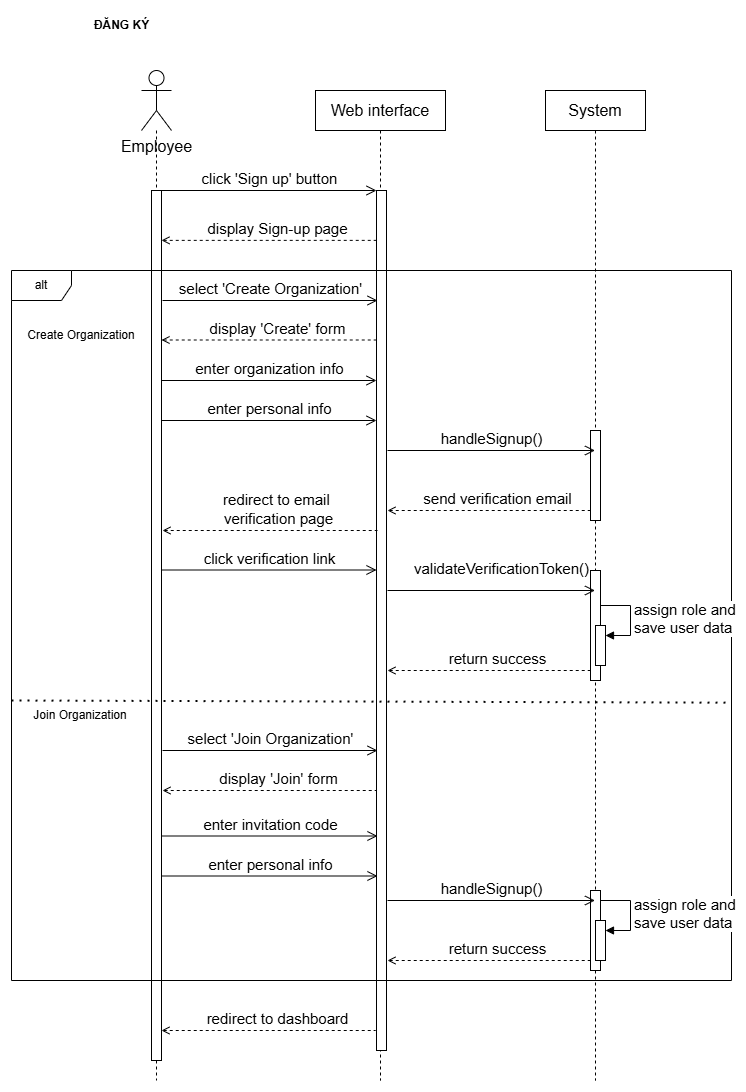
\includegraphics[width=1\textwidth]{Dg_Sequence/Sequence Diagram-Signup.png}
	\vspace{0.5cm}
	\caption{Biểu đồ sequence cho Đăng ký}
	\label{fig:enter-label}
\end{figure}

\subsubsubsection{Đăng nhập}
Hình 38 biểu diễn biểu đồ tuần tự cho tính năng Đăng nhập.

\textbf{Mô tả}: Biểu đồ tuần tự Đăng nhập mô tả sự tương tác giữa các thực thể sau:
\begin{itemize}
	\item Actor: Nhân viên (gồm cả quản trị viên và nhân viên chăm sóc khách hàng).
	\item Giao diện trang web (Web interface).
	\item Hệ thống.
\end{itemize}
Các bước trong quá trình tương tác như sau:
\begin{enumerate}
	\item Nhân viên ấn nút Đăng nhập.
	\item Giao diện hiển thị trang Đăng nhập.
	
	% \textbf{Trường hợp sử dụng tài khoản và mật khẩu:}
	% \begin{enumerate}
		\item Nhân viên nhập hai thông tin trên. Sau đó ấn nút "Đăng nhập" để gọi phương thức onClickLoginButton() trên giao diện. 
		\item Phương thức handleSignInByAccount() của hệ thống được gọi.
		\item Hệ thống trả về mã thông báo thành công cho giao diện web.
		\item Nhân viên được điều hướng về trang chủ.
	% \end{enumerate}
	
	% \textbf{Trường hợp sử dụng Google OAuth:}
	% \begin{enumerate}
	% 	\item Nhân viên ấn nút "Tiếp tục với Google" để gọi phương thức onClickGoogleButton() trên giao diện. 
	% 	\item Phương thức handleSignInByGoogle() của hệ thống được gọi.
	% 	\item Hàm verifyGmail() của Google OAuth được gọi, và một yêu cầu ủy quyền được gửi đến giao diện người dùng.
	% 	\item Nhân viên chọn "Đồng ý" (gọi phương thức onClickToAuthorize()) để ủy quyền.
	% 	\item OAuth trả về thông tin truy vấn cho hệ thống.
	% 	\item Hệ thống dùng thông tin này để gọi phương thức getTokens() từ OAuth.
	% 	\item OAuth trả về id\_token và refresh\_token cho hệ thống.
	% 	\item Hệ thống dùng các token này để gọi phương thức getUserInfo() từ OAuth.
	% 	\item OAuth trả về thông tin người dùng cho hệ thống.
	% 	\item Hệ thống dùng các thông tin này để tạo token đăng nhập (CreateLoginTokens()) và đăng nhập (LoginByTokens())
	% 	\item Hệ thống trả về thông báo thành công cho giao diện người dùng.
	% 	\item Nhân viên được điều hướng về trang chủ.
	% \end{enumerate}
\end{enumerate}

\begin{figure}[H]
	\centering
	\includesvg[width=0.6\textwidth]{Dg_Sequence/Sequence Diagram-Login.svg}
	\vspace{0.5cm}
	\caption{Biểu đồ sequence cho Đăng nhập}
	\label{fig:enter-label}
\end{figure}




\subsubsubsection{Chỉnh sửa hồ sơ cá nhân}
Hình 39 biểu diễn biểu đồ tuần tự cho tính năng Chỉnh sửa hồ sơ cá nhân.

\textbf{Mô tả}: Biểu đồ tuần tự Chỉnh sửa hồ sơ cá nhân mô tả sự tương tác giữa các thực thể sau:
\begin{itemize}
	\item Actor: Nhân viên (gồm cả quản trị viên và nhân viên chăm sóc khách hàng).
	\item Giao diện trang web (Web interface).
	\item Hệ thống.
	\item Database.
\end{itemize}
Các bước trong quá trình tương tác như sau:
\begin{enumerate}
	\item Nhân viên ấn nút "Cài đặt".
	\item Giao diện hiển thị trang Cài đặt. Nhân viên ấn vào mục Tài khoản.
	
	\textbf{Trường hợp chỉnh sửa thông tin cá nhân:}
	\begin{enumerate}
		\item Nhân viên chỉnh sửa các thông tin: ảnh đại diện, họ tên, số điện thoại và ấn nút "Đăng nhập" để gọi phương thức onClickSaveButton() trên giao diện. 
		\item Phương thức onSaveNewInfo(newInfo) của hệ thống được gọi.
		\item Các lệnh update được thực hiện trong cơ sở dữ liệu.
		\item Mã thông báo thành công được trả về, các thông tin mới được hiển thị lên giao diện web.
	\end{enumerate}
	
	\textbf{Trường hợp sử dụng thay đổi mật khẩu:}
	\begin{enumerate}
		\item Nhân viên nhập mật khẩu hiện tại, mật khẩu mới và ấn "Lưu" để gọi phương thức onClickSaveButton() trên giao diện. 
		\item Phương thức handleSaveNewPwd() của hệ thống được gọi.
		\item Hệ thống kiểm tra mật khẩu hiện tại đã đúng chưa (VerifyCurrentPwd()).
		\item Mã thông báo thành công được trả về.
		\item Giao diện web hiển thị thông báo thành công.
	\end{enumerate}
\end{enumerate}

\begin{figure}[H]
	\centering
	\includesvg[width=1\textwidth]{Dg_Sequence/Sequence Diagram-Profile.svg}
	\vspace{0.5cm}
	\caption{Biểu đồ sequence cho Chỉnh sửa hồ sơ cá nhân}
	\label{fig:enter-label}
\end{figure}



\subsubsection{Đào tạo và tùy chỉnh chatbot}
\subsubsubsection{Đào tạo chatbot}
Hình 40, 41 và 42 biểu diễn biểu đồ tuần tự cho tính năng Đào tạo chatbot.

\textbf{Mô tả}: Biểu đồ tuần tự Đào tạo chatbot mô tả sự tương tác giữa các thực thể sau:
\begin{itemize}
	\item Actor: Nhân viên quản lý (chủ sở hữu/quản trị viên).
	\item Giao diện trang web (trang chatbot training).
	\item Hệ thống.
	\item Thiết bị.
\end{itemize}
Các bước trong quá trình tương tác như sau:
\begin{enumerate}
	\item Người dùng mở trang Đào tạo chatbot, khi đó Hệ thống sẽ gọi getDocuments() và trả về giao diện danh sách các tri thức.
	\item Tiếp theo người dùng có thể thực hiện nhiều lần các lựa chọn sau:
	\begin{itemize}
		\item Xóa tri thức: người dùng chọn delete cho tri thức có id trên màn hình. Giao diện hiển thị confirmModal. Nếu người dùng chọn xác nhận, hệ thống gọi delete(id) để xóa tri thức, khi đó hệ thống sẽ gọi checkStatus(id) để kiểm tra trạng thái, nếu untrained thì gọi permanentDelete(id), còn không gọi temporaryDelete(id) sau đó sẽ trả về thông báo thành công. Nếu người dùng chọn Hủy, giao diện đóng modal và kết thúc.
		\item Thêm tri thức: Người dùng mở Cập nhật tri thức. Khi đó có 3 lựa chọn để thêm tri thức:
		\begin{itemize}
			\item Tập tin: Người dùng nhấn tải file, thiết bị người dùng gọi displayFile() và trả files về giao diện. Người dùng chọn các file cần tải lên, thiết bị gọi hàm selectFiles(files) để chọn file và trả files là các file đã chọn. Người dùng có thể xóa các file đã tải và cuối cùng lưu, giao diện gọi onSubmit(files), hệ thống gọi addDocument(files) và trả về thông báo thành công.
			\item Văn bản: Người dùng mở tab thêm tri thức, điền và lưu, giao diện gọi onSubmit(text), hệ thống gọi addDocument(text) và trả về thông báo thành công.
			\item Website: Người dùng mở tab thêm tri thức web, điền thông tin và lưu, giao diện gọi onSubmit(infos), hệ thống gọi addDocument(infos) và trả về thông báo thành công. 
		\end{itemize}
		\item Sửa độ ưu tiên: người dùng sửa độ ưu tiên cho tri thức, giao diện gọi onChange(id, priority) với id là id của tri thức, priority là độ ưu tiên mới.
	\end{itemize}
	\item Sau khi hoàn thành quá trình chỉnh sửa, người dùng chọn Lưu và đào tạo. Trước hết, nếu tồn tại tri thức bị xóa tạm thời, hệ thống gọi permanentDelete(ids) để xóa các tri thức. Nếu tồn tại sự thay đổi độ ưu tiên, hệ thống gọi changePriority(ids, priorities) để đổi độ ưu tiên mới, sau đó hệ thống sẽ gọi hàm train() để bắt đầu đào tạo và pendingTrain() để đặt trạng thái chờ. Khi xong, hệ thống trả về thông báo thành công.
\end{enumerate}

\begin{figure}[H]
	\centering
	\includesvg[width=1\textwidth]{Dg_Sequence/daotao.svg}
	\vspace{0.5cm}
	\caption{Biểu đồ sequence cho Đào tạo chatbot}
	\label{fig:enter-label}
\end{figure}

\begin{figure}[H]
	\centering
	\includesvg[width=1\textwidth]{Dg_Sequence/xoatrithuc.svg}
	\vspace{0.5cm}
	\caption{Biểu đồ sequence cho Xóa tri thức}
	\label{fig:enter-label}
\end{figure}

\subsubsubsection{Tùy chỉnh chatbot}
Hình 43 biểu diễn biểu đồ tuần tự cho tính năng Tùy chỉnh chatbot.

\textbf{Mô tả}: Biểu đồ tuần tự Tùy chỉnh chatbot mô tả sự tương tác giữa các thực thể sau:
\begin{itemize}
	\item Actor: Nhân viên quản lý (chủ sở hữu/quản trị viên).
	\item Giao diện trang web (trang tùy chỉnh chatbot).
	\item Hệ thống.
	\item Thiết bị.
\end{itemize}
Các bước trong quá trình tương tác như sau: 

\begin{enumerate}
	\item Đầu tiên quản trị viên vào mục Tùy chỉnh chatbot. Khi đó hệ thống sẽ gọi hàm getConfigs() để lấy cấu hình hiện tại và trả về cho giao diện. 
	\item Tiếp theo người dùng có 2 lựa chọn:
	\begin{itemize}
		\item Chỉnh sửa giao diện: Người dùng có thể thực hiện các lựa chọn sau nhiều lần.
		\begin{itemize}
			\item Đổi ảnh: Người dùng chọn tải file, hệ thống gọi displayFile() và các về các files hợp lệ. Người dùng chọn file, hệ thống gọi selectFile(file) và trả về file được chọn lên giao diện.
			\item Đổi thông tin: Người dùng thay đổi thông tin của một thành phần giao diện onChange(value).
		\end{itemize}
		Tiếp đến nếu không chỉnh sửa gì thêm, người dùng có thể xem trước giao diện, hệ thống gọi preview(configs) với configs là cấu hình đã sửa và trả về previewInterface.

		Cuối cùng người dùng có 2 lựa chọn:
		\begin{itemize}
			\item Lưu: chọn Lưu, hệ thống save(configs) và trả về thông báo thành công.
			\item Hủy: chọn Hủy, giao diện gọi reset() để khôi phục lại cấu hình hiện tại.
		\end{itemize}
		\item Chỉnh sửa phong cách: Người dùng tiếp tục có 2 lựa chọn:
		\begin{itemize}
			\item Tông giọng: Người dùng thay đổi tông giọng, hệ thống gọi change(tone) và trả về thông báo thành công.
			\item Tin nhắn mặc định: Người dùng chọn loại tin nhắn và điền nội dung. Nếu người dùng chọn Lưu, hệ thống gọi change(type, message) (với type là loại tin nhắn, message là nội dung mới) và trả về thông báo thành công. Nếu hủy, giao diện reset() để khôi phục lại giá trị hiện tại.
		\end{itemize}
	\end{itemize}
\end{enumerate}

\begin{figure}[H]
	\centering
	\includesvg[width=1\textwidth]{Dg_Sequence/themtrithuc.svg}
	\vspace{0.5cm}
	\caption{Biểu đồ sequence cho Thêm tri thức}
	\label{fig:enter-label}
\end{figure}



% \subsubsubsection{Tải dữ liệu tri thức}
% \begin{figure}[H]
% 	\centering
% 	\includesvg[width=1\textwidth]{Dg_Sequence/Sequence Diagram-LoadKnowledge.svg}
% 	\vspace{0.5cm}
% 	\caption{Biểu đồ sequence cho Tải dữ liệu tri thức}
% 	\label{fig:enter-label}
% \end{figure}

% \textbf{Mô tả}: Biểu đồ tuần tự Tải dữ liệu tri thức mô tả sự tương tác giữa các thực thể sau:
% \begin{itemize}
% 	\item Actor: Quản trị viên.
% 	\item Giao diện trang web (Web interface).
% 	\item Hệ thống.
% 	\item Cơ sở dữ liệu.
% \end{itemize}
% Các bước trong quá trình tương tác như sau:
% \begin{enumerate}
% 	\item Nhân viên ấn vào tab "Cập nhật tri thức" của mục "Đào tạo Chatbot". (gọi phương thức openUpdateKnowledgeTab())
% 	\item Giao diện hiển thị trang tab Cập nhật tri thức.
% 	\item Sau khi điền thông tin cần thiết, nhân viên tải file lên. (onClickFileButton() > handleLoadFile())
% 	\item Một yêu cầu xử lý (phương thức verifyFileType() của hệ thống) được gọi. Hàm này chọn ra các file có định dạng phù hợp.
% 	\item Các file được chấp nhận sẽ được chèn vào cơ sở dữ liệu, mã kết quả insert được trả về.
% 	\item Hệ thống gửi mã thông báo thành công về giao diện web.
% 	\item Giao diện hiển thị các file đã tải lên thành công.
% \end{enumerate}

% \subsubsubsection{Cập nhật dữ liệu tri thức}
% \begin{figure}[H]
% 	\centering
% 	\includesvg[width=1\textwidth]{Dg_Sequence/Sequence Diagram-UpdateKnowledge.svg}
% 	\vspace{0.5cm}
% 	\caption{Biểu đồ sequence cho Cập nhật dữ liệu tri thức}
% 	\label{fig:enter-label}
% \end{figure}

% \textbf{Mô tả}: Biểu đồ tuần tự Cập nhật dữ liệu tri thức mô tả sự tương tác giữa các thực thể sau:
% \begin{itemize}
% 	\item Actor: Quản trị viên.
% 	\item Giao diện trang web (Web interface).
% 	\item Hệ thống.
% 	\item Cơ sở dữ liệu.
% \end{itemize}
% Các bước trong quá trình tương tác như sau:
% \begin{enumerate}
% 	\item Nhân viên ấn vào tab "Cập nhật tri thức" của mục "Đào tạo Chatbot". (gọi phương thức openUpdateKnowledgeTab())
% 	\item Giao diện hiển thị trang tab Cập nhật tri thức.
% 	\item Chọn file cần xóa (onClickDelete(fileID) trên giao diện web.)
% 	\item Một yêu cầu xử lý (phương thức onDeleteFile(fileID) của hệ thống) được gọi để xóa tệp này.
% 	\item Các truy vấn xóa được thực hiện trong cơ sở dữ liệu, trả về kết quả.
% 	\item Hệ thống gửi mã thông báo thành công về giao diện web.
% 	\item Giao diện hiển thị các file hiện có.
% \end{enumerate}
% Trường hợp quản trị viên muốn cập nhật websites, tham chiếu đến Biểu đồ tuần tự Cập nhật websites; tương tự, khi cập nhật tài liệu hướng dẫn tham chiếu đến Biểu đồ tuần tự Cập nhật hướng dẫn.

% \begin{figure}[H]
% 	\centering
% 	\includesvg[width=1\textwidth]{Dg_Sequence/Sequence Diagram-UpdateWeb.svg}
% 	\vspace{0.5cm}
% 	\caption{Biểu đồ sequence cho Cập nhật websites}
% 	\label{fig:enter-label}
% \end{figure}

% \textbf{Mô tả}: Biểu đồ tuần tự Cập nhật websites mô tả sự tương tác giữa các thực thể sau:
% \begin{itemize}
% 	\item Actor: Quản trị viên.
% 	\item Giao diện trang web (Web interface).
% 	\item Hệ thống.
% 	\item Cơ sở dữ liệu.
% \end{itemize}
% Các bước trong quá trình tương tác như sau:
% \begin{enumerate}
% 	\item \textbf{Trường hợp cần xóa trang web:}
% 	\begin{enumerate}
% 		\item Người dùng chọn trang web cần xóa (gọi onDeleteWeb(address) của giao diện web).
% 		\item Lời gọi onDeleteWeb(address) từ hệ thống để xóa trang web mục tiêu.
% 		\item Các câu truy vấn xóa được thực hiện trong cơ sở dữ liệu và trả về thông tin kết quả.
% 		\item Mã thông báo thành công được trả về cho giao diện web.
% 	\end{enumerate}
% 	\item \textbf{Trường hợp cần sửa địa chỉ web:}
% 	\begin{enumerate}
% 		\item Người dùng chọn địa chỉ web cần sửa (gọi onChangeCurrentWeb(newaddress) của giao diện web).
% 		\item Lời gọi onChangeCurrentWeb(currentID, newaddress) từ hệ thống để chỉnh sửa trang web mục tiêu.
% 		\item Hệ thống tiếp tục dùng phương thức verifyAddress(newAddress) để kiểm tra sự hợp lệ của địa chỉ.
% 		\item Các câu truy vấn cập nhật được thực hiện trong cơ sở dữ liệu và trả về thông tin kết quả.
% 		\item Mã thông báo thành công được trả về cho giao diện web.
% 	\end{enumerate}
% \end{enumerate}

% Cuối cùng, giao diện cập nhật hiển thị các trang web hiện có.

% \begin{figure}[H]
% 	\centering
% 	\includesvg[width=1\textwidth]{Dg_Sequence/Sequence Diagram-UpdateNote.svg}
% 	\vspace{0.5cm}
% 	\caption{Biểu đồ sequence cho Cập nhật hướng dẫn}
% 	\label{fig:enter-label}
% \end{figure}

% \textbf{Mô tả}: Biểu đồ tuần tự Cập nhật websites mô tả sự tương tác giữa các thực thể sau:
% \begin{itemize}
% 	\item Actor: Quản trị viên.
% 	\item Giao diện trang web (Web interface).
% 	\item Hệ thống.
% 	\item Cơ sở dữ liệu.
% \end{itemize}
% Các bước trong quá trình tương tác như sau:
% \begin{enumerate}
% 	\item \textbf{Trường hợp cần xóa hướng dẫn:}
% 	\begin{enumerate}
% 		\item Người dùng chọn trang web cần xóa (gọi onDeleteNote(noteID) của giao diện web).
% 		\item Lời gọi onDeleteNote(noteID) từ hệ thống để xóa trang web mục tiêu.
% 		\item Các câu truy vấn xóa được thực hiện trong cơ sở dữ liệu và trả về thông tin kết quả.
% 		\item Mã thông báo thành công được trả về cho giao diện web.
% 	\end{enumerate}
% 	\item \textbf{Trường hợp cần sửa địa chỉ web:}
% 	\begin{enumerate}
% 		\item Người dùng chọn hướng dẫn cần sửa (gọi onChangeCurrentWeb(newcontent) của giao diện web).
% 		\item Lời gọi onChangeNote(noteID, newcontent) từ hệ thống để chỉnh sửa hướng dẫn.
% 		\item Các câu truy vấn cập nhật được thực hiện trong cơ sở dữ liệu và trả về thông tin kết quả.
% 		\item Mã thông báo thành công được trả về cho giao diện web.
% 	\end{enumerate}
% \end{enumerate}

% Cuối cùng, giao diện cập nhật hiển thị các hướng dẫn hiện có.


% \subsubsubsection{Gán nhãn dữ liệu tri thức}
% \begin{figure}[H]
% 	\centering
% 	\includesvg[width=1\textwidth]{Dg_Sequence/Sequence Diagram-LabelKnowledge.svg}
% 	\vspace{0.5cm}
% 	\caption{Biểu đồ sequence cho Gán nhãn dữ liệu tri thức}
% 	\label{fig:enter-label}
% \end{figure}
% \textbf{Mô tả}: Biểu đồ tuần tự Gán nhãn dữ liệu tri thức mô tả sự tương tác giữa các thực thể sau:
% \begin{itemize}
% 	\item Actor: Quản trị viên.
% 	\item Giao diện trang web (Web interface).
% 	\item Hệ thống.
% 	\item Cơ sở dữ liệu.
% \end{itemize}
% Các bước trong quá trình tương tác như sau:
% \begin{enumerate}
% 	\item Nhân viên ấn vào tab "Gán nhãn tri thức" của mục "Đào tạo Chatbot". (gọi phương thức openLabelKnowledgeTab())
% 	\item Giao diện hiển thị trang tab Gán nhãn tri thức.
% 	\item Quản trị viên lựa chọn hạng mục cho file tải lên qua bảng chọn select. (onDropSelection(file, topic))
% 	\item Một yêu cầu xử lý (phương thức onAssignTopic(fileID, topic) của hệ thống) được gọi. 
% 	\item Hạng mục của file được cập nhật vào cơ sở dữ liệu, kết quả update được trả về.
% 	\item Hệ thống gửi mã thông báo thành công về giao diện web.
% 	\item Giao diện hiển thị hạng mục mới của file.
% \end{enumerate}

% \subsubsubsection{So sánh chatbot}
% \begin{figure}[H]
% 	\centering
% 	\includesvg[width=1\textwidth]{Dg_Sequence/Sequence Diagram-Compare.svg}
% 	\vspace{0.5cm}
% 	\caption{Biểu đồ sequence cho So sánh chatbot}
% 	\label{fig:enter-label}
% \end{figure}

% \textbf{Mô tả}: Biểu đồ tuần tự So sánh chatbot mô tả sự tương tác giữa các thực thể sau:
% \begin{itemize}
% 	\item Actor: Quản trị viên.
% 	\item Giao diện trang web (Web interface).
% 	\item Hệ thống.
% 	\item Cơ sở dữ liệu.
% \end{itemize}
% Các bước trong quá trình tương tác như sau:
% \begin{enumerate}
% 	\item Nhân viên ấn vào tab "Gán nhãn tri thức" của mục "Đào tạo Chatbot". (gọi phương thức openLabelKnowledgeTab())
% 	\item Giao diện hiển thị trang tab Gán nhãn tri thức.
% 	\item Quản trị viên ấn vào nút "So sánh chatbot". (onPreviewVersions() của giao diện)
% 	\item Một yêu cầu xử lý (phương thức onLoadBots() của hệ thống) được gọi. 
% 	\item Các tài liệu cũng như cấu hình được truy vấn trong cơ sở dữ liệu, sau đó được gửi về hệ thống.
% 	\item Hệ thống gửi các cấu hình về giao diện web.
% 	\item Giao diện hiển thị hai phiên bản của bot.
% 	\item Người dùng nhập câu hỏi để hai bot trả lời (gọi phương thức onAskQuestion(question) của giao diện)
% 	\item Phương thức onGenAnswers(question) của hệ thống được gọi và trả về câu trả lời cho trang web.
% 	\item Hai câu trả lời được hiển thị trên giao diện.
% 	\item Quản trị viên ấn "Lưu và training" để gọi phương thức onSaveBot() của giao diện.
% 	\item Lời gọi onSaveBot() của hệ thống sau đó được thực hiện
% 	\item Các lệnh truy vấn xóa các dữ liệu cũ, cập nhật được thực hiện và trả về kết quả cho hệ thống.
% 	\item Kết quả được trả về tiếp tục cho giao diện web, đồng thời khóa nút "So sánh chatbot" (disableButton(previewBtn))
%  \end{enumerate}



\begin{figure}[H]
	\centering
	\includesvg[width=1\textwidth]{Dg_Sequence/Sequence Diagram-AdjustBot.svg}
	\vspace{0.5cm}
	\caption{Biểu đồ sequence cho Tùy chỉnh chatbot}
	\label{fig:enter-label}
\end{figure}


\subsubsection{Quản lý chatbot}
\subsubsubsection{Báo cáo}
Hình 44 biểu diễn biểu đồ tuần tự cho tính năng Báo cáo.

\textbf{Mô tả: }
\begin{itemize}
	\item Quản trị viên doanh nghiệp mở trang Báo cáo qua hàm onOpen(report).
	\item Giao diện trang Báo cáo sẽ gọi hàm getStatistics() đến Hệ thống để lấy các dữ liệu thống kê.
	\item Hệ thống phản hồi và trả lại các dữ liệu thống kê cho trang Báo cáo.
	\item Có 2 tùy chọn khả dụng là quản trị viên có thể chọn lọc hoặc xuất:
	\begin{itemize}
		\item Lọc: quản trị viên click nút Lọc với onClickFilterButton(), trang Báo cáo gọi hàm getFilterFields() và hiển thị các trường lọc, quản trị viên tiếp tục chọn trường cần lọc với onClickFilterField(field) có biến field truyền vào, trang Báo cáo gọi hàm getStatistics(field) đến hệ thống để lấy dữ liệu thống kê theo trường lọc đó, hệ thống trả lại các figuresAndCharts tương ứng.
		\item Xuất: quản trị viên click nút Xuất với onClickExportButton(), trang Báo cáo gọi hàm getFileTypes() và hiển thị các loại file, quản trị viên tiếp tục chọn loại file với onClickFileType(type) có biến type được truyền vào, hệ thống gọi hàm downloadFile(type) lên thiết bị để file được tải xuống thiết bị, khi thành công thiết bị trả tin nhắn thành công lại trang báo cáo.
	\end{itemize}
\end{itemize}

\begin{figure}[H]
    \centering
     \includesvg[width=1\textwidth]{Dg_Sequence/Sequence Diagram-Report.svg}
    \vspace{0.5cm}
    \caption{Biểu đồ sequence cho Báo cáo}
    \label{fig:enter-label}
\end{figure}

\subsubsubsection{Lịch sử hội thoại}
Hình 45 biểu diễn biểu đồ tuần tự cho tính năng Lịch sử hội thoại.

\textbf{Mô tả: }
\begin{itemize}
	\item Nhân viên doanh nghiệp mở trang Hội thoại qua hàm onOpen(chat).
	\item Giao diện trang Hội thoại sẽ gọi hàm getChats() đến Hệ thống để lấy danh sách các cuộc hội thoại.
	\item Hệ thống phản hồi và trả lại danh sách các cuộc hội thoại cho trang Hội thoại.
	\item Có 3 tùy chọn khả dụng là nhân viên có thể chọn lọc, tìm kiếm hoặc chọn xem các cuộc hội thoại cần hỗ trợ:
	\begin{itemize}
		\item Lọc: nhân viên click nút Lọc với onClickFilterButton(), trang Hội thoại hiển thị các trường lọc, nhân viên tiếp tục chọn trường cần lọc với onClickFilterField(field) có biến field truyền vào, trang Hội thoại gọi hàm getChats(field) đến hệ thống để lấy dữ liệu hội thoại theo trường lọc đó, hệ thống trả lại các chats tương ứng.
		\item Tìm kiếm: nhân viên click khung Search với onClickSearchBox(), tiếp tục nhập và hoàn thành nội dung tìm kiếm với submit(searchInput), trang Hội thoại gọi hàm getChats(searchInput) đế hệ thống với biến searchInput từ nhân viên truyền tới để lấy dữ liệu hội thoại theo nội dung tìm kiếm đó, hệ thống trả lại các chats tương ứng.
		\item Xem các cuộc hội thoại cần hỗ trợ: nhân viên click nút Cần hỗ trợ với onClickNeedSupportBtn(), trang Hội thoại gọi hàm getChats(needSupport) đến hệ thống để lấy danh sách các cuộc hội thoại cần hỗ trợ, hệ thống trả lại các chats tương ứng.
	\end{itemize}
	\item Nhân viên tiếp tục chọn xem 1 cuộc hội thoại với onClickChatItem(id).
	\item Trang Hội thoại gọi hàm getChat(id) đến hệ thống với biến id truyền vào.
	\item Hệ thống trả lại chat tương ứng.
\end{itemize}

\begin{figure}[H]
    \centering
     \includesvg[width=1\textwidth]{Dg_Sequence/Sequence Diagram-Chat.svg}
    \vspace{0.5cm}
    \caption{Biểu đồ sequence cho Lịch sử hội thoại}
    \label{fig:enter-label}
\end{figure}

\subsubsection{Quản lý thanh toán}
Hình 46 biểu diễn biểu đồ tuần tự cho tính năng Quản lý thanh toán.

\textbf{Mô tả: }
\begin{itemize}
	\item Người dùng điều hướng đến trang thanh toán.
	\item Trang thanh toán sẽ gọi hàm getAvailablePlan() đến hệ thống để lấy các gói dịch vụ.
	\item Hệ thống trả về danh sách các gói dịch vụ và hiển thị với người dùng.
	\item Người dùng chọn một gói dịch vụ.
	\item Trang thanh toán gọi hàm selectPlan() đến hệ thống.
	\item Hệ thống gọi hàm initiatePayment() đến hệ thống thanh toán.
	\item Hệ thống thanh toán trả về trang thanh toán và hiển thị với người dùng.
	\item Người dùng có 2 lựa chọn:
	\begin{itemize}
		\item Thanh toán: người dùng quét mã QR để thanh toán, hệ thống thanh toán tự gọi hàm processPayment() để tiến hành quá trình thanh toán và thành công thì trả về thông báo thành công.
		\item Hủy: Người dùng hủy thanh toán, hệ thống gọi hàm cancel() và trả về thông báo hủy thành công.
	\end{itemize}
\end{itemize}

\begin{figure}[H]
    \centering
     \includesvg[width=1\textwidth]{Dg_Sequence/Payment.svg}
    \vspace{0.5cm}
    \caption{Biểu đồ sequence cho Quản lý thanh toán}
    \label{fig:enter-label}
\end{figure}

\subsubsection{Tương tác với chatbot}
\subsubsubsection{Phản hồi tin nhắn khách hàng}
Hình 47 biểu diễn biểu đồ tuần tự cho tính năng Phản hồi tin nhắn khách hàng.

\textbf{Mô tả: }
\begin{itemize}
	\item Nhân viên CSKH chọn xem 1 cuộc hội thoại với onClickChatItem(id).
	\item Trang Hội thoại gọi hàm getChat(id) đến hệ thống với biến id truyền vào.
	\item Hệ thống trả lại chat tương ứng.
	\item Có một vòng lặp với điều kiện nhân viên CSKH tiếp tục quá trình nhập tin nhắn: nhân viên CSKH click vào khung tin nhắn với onClickMessageBox(), tiếp tục nhập nội dung tin nhắn với enter(messageInput) có biến messageInput truyền vào.
	\item Có một tùy chọn với điều kiện tin nhắn tồn tại: nhân viên CSKH click Gửi với onClickSendButton(), trang Hội thoại gọi hàm sendMessage() đến hệ thống, hệ thống trả lại tin nhắn sentMessage tương ứng.
\end{itemize}

\begin{figure}[H]
    \centering
     \includesvg[width=1\textwidth]{Dg_Sequence/Sequence Diagram-ReplyCustomerMessage.svg}
    \vspace{0.5cm}
    \caption{Biểu đồ sequence cho Phản hồi tin nhắn khách hàng}
    \label{fig:enter-label}
\end{figure}

\subsubsubsection{Gửi tin nhắn}
Hình 48 biểu diễn biểu đồ tuần tự cho tính năng Gửi tin nhắn.

\begin{figure}[H]
    \centering
     \includesvg[width=1\textwidth]{Dg_Sequence/Sequence Diagram-SendMessage.svg}
    \vspace{0.5cm}
    \caption{Biểu đồ sequence cho Gửi tin nhắn}
    \label{fig:enter-label}
\end{figure}


\textbf{Mô tả: }
\begin{itemize}
	\item Khách hàng click vào nút Chatbot với onOpenChatbotPopup().
	\item Giao diện gọi hàm getChat(id) đến hệ thống với biến id truyền vào.
	\item Hệ thống trả lại chat tương ứng.
	\item Có một vòng lặp với điều kiện khách hàng tiếp tục quá trình nhập tin nhắn: khách hàng click vào khung tin nhắn với onClickMessageBox(), tiếp tục nhập nội dung tin nhắn với enter(messageInput) có biến messageInput truyền vào.
	\item Có một tùy chọn với điều kiện tin nhắn tồn tại: khách hàng click Gửi với onClickSendButton(), giao diện gọi hàm sendMessage() đến hệ thống, hệ thống trả lại tin nhắn sentMessage tương ứng, hệ thống tự gọi hàm createAutoReplyMessage() để tạo tin nhắn tự động từ hệ thống chatbot, hệ thống trả lại giao diện autoReplyMessage.
\end{itemize}



\subsubsubsection{Yêu cầu hỗ trợ}
Hình 49 biểu diễn biểu đồ tuần tự cho tính năng Yêu cầu hỗ trợ.

\begin{figure}[H]
    \centering
     \includesvg[width=1\textwidth]{Dg_Sequence/Sequence Diagram-NeedSupport.svg}
    \vspace{0.5cm}
    \caption{Biểu đồ sequence cho Yêu cầu hỗ trợ}
    \label{fig:enter-label}
\end{figure}
\textbf{Mô tả: }
\begin{itemize}
	\item Khách hàng click nút Hỗ trợ với hàm onOpenSupportPoppup().
	\item Giao diện gọi hàm getSupportInro() đế hệ thống để lấy thông tin hỗ trợ.
	\item Hệ thống trả về giao diện supportInfo.
	\item Có 2 tùy chọn khả dụng là gửi yêu cầu hỗ trợ hoặc hủy:
	\begin{itemize}
		\item Gửi yêu cầu hỗ trợ: khách hàng nhập thông tin và chọn lưu với onSubmit(info), hệ thống gọi sendRequest(info) để đặt chế độ hỗ trợ cho đoạn chat và gọi stopAutoReply() để tắt chế độ tự động chat.
		\item Hủy: khách hàng chọn Hủy, giao diện đóng cửa sổ hỗ trợ với closeSupportPopup()
	\end{itemize}
\end{itemize}
% \subsubsection{Quản lý lịch hẹn}
% \begin{figure}[H]
%     \centering
%      \includesvg[width=1\textwidth]{Dg_Sequence/Sequence Diagram-AppointmentManagement.svg}
%     \vspace{0.5cm}
%     \caption{Biểu đồ sequence cho Quản lý lịch hẹn}
%     \label{fig:enter-label}
% \end{figure}
% \textbf{Mô tả: }
% \begin{itemize}
% 	\item Nhân viên CSKH mở trang Lịch hẹn qua hàm onOpen(appointment).
% 	\item Giao diện trang Lịch hẹn sẽ gọi hàm getAppointments() đến Hệ thống để lấy danh sách các lịch hẹn.
% 	\item Hệ thống phản hồi và trả lại danh sách các lịch hẹn cho trang Lịch hẹn.
% 	\item Có 3 tùy chọn khả dụng là nhân viên CSKH có thể chọn lọc hoặc tìm kiếm lịch hẹn:
% 	\begin{itemize}
% 		\item Lọc: nhân viên CSKH click nút Lọc với onClickFilterButton(), trang Lịch hẹn gọi hàm getFilterFields() đến hệ thống, hệ thống trả lại dữ liệu các filterFields, nhân viên CSKH tiếp tục chọn trường cần lọc với onClickFilterField(field) có biến field truyền vào, trang Lịch hẹn gọi hàm getAppointments(field) đến hệ thống để lấy dữ liệu lịch hẹn theo trường lọc đó, hệ thống trả lại các appointments tương ứng.
% 		\item Tìm kiếm: nhân viên CSKH click khung Search với onClickSearchBox(), tiếp tục nhập và hoàn thành nội dung tìm kiếm với submit(searchInput), trang Lịch hẹn gọi hàm getAppointments(searchInput) đế hệ thống với biến searchInput từ nhân viên CSKH truyền tới để lấy dữ liệu lịch hẹn theo nội dung tìm kiếm đó, hệ thống trả lại các appointments tương ứng.
% 	\end{itemize}
% 	\item Nhân viên CSKH tiếp tục chọn xem 1 lịch hẹn với onClickChatItem(id).
% 	\item Trang Lịch hẹn gọi hàm getAppointment(id) đến hệ thống với biến id truyền vào.
% 	\item Hệ thống trả lại appointment tương ứng.
% 	\item Có một tùy chọn với điều kiện nhân viên CSKH muốn hỗ trợ khách hàng: nhân viên CSKH click Hỗ trợ với onClickSupportButton(), trang Lịch hẹn gọi switchToChatPage(id) đến hệ thống với biến id để mở trang hội thoại tương ứng, hệ thống mở trang Hội thoại với onOpen(chat), trang Hội thoại gọi hàm getChat(id) để lấy thông tin cuộc hội thoại, hệ thống trả về chat tương ứng.
% \end{itemize}
